% Created 2020-01-15 Ср 09:05
% Intended LaTeX compiler: pdflatex
\documentclass[presentation]{beamer}
\usepackage[utf8]{inputenc}
\usepackage[T1]{fontenc}
\usepackage{graphicx}
\usepackage{grffile}
\usepackage{longtable}
\usepackage{wrapfig}
\usepackage{rotating}
\usepackage[normalem]{ulem}
\usepackage{amsmath}
\usepackage{textcomp}
\usepackage{amssymb}
\usepackage{capt-of}
\usepackage{hyperref}
\usetheme{default}
\author{pasha}
\date{\today}
\title{Обзор систем авторизации OAuth + UMA Protocol flow}
\hypersetup{
 pdfauthor={pasha},
 pdftitle={Обзор систем авторизации OAuth + UMA Protocol flow},
 pdfkeywords={},
 pdfsubject={},
 pdfcreator={Emacs 26.3 (Org mode 9.3)},
 pdflang={English}}
\begin{document}

\maketitle
\begin{frame}{Outline}
\tableofcontents
\end{frame}


\begin{frame}[label={sec:org24b9295},fragile]{Решения авторизации}
 \begin{block}{Shiro}
\begin{itemize}
\item Сайт: \url{https://shiro.apache.org}
\item Java, лицензия Apache2
\item OAuth2 поддерживается отдельным решением: \url{https://github.com/bujiio/buji-pac4j}
\item Источник данных о пользователях - любой: для этого надо реализовать интерфейс \href{https://shiro.apache.org/realm.html}{Realm}.
\item Хорошая документация
\item RBAC и item-based permissions
\end{itemize}

\begin{block}{Механизм аутентификации}
\alert{Subject} - принятый термин для пользователя

\begin{center}
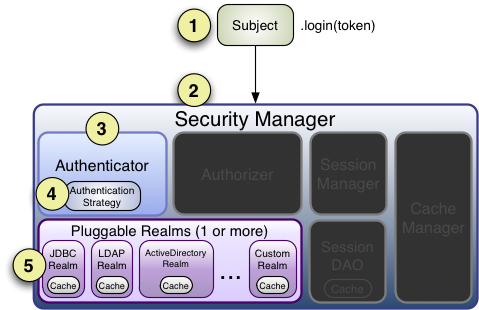
\includegraphics[width=.9\linewidth]{./img/ShiroAuthenticationSequence.png}
\end{center}

\begin{enumerate}
\item Приложение вызывает \texttt{Subject.login} с аргументом типа \texttt{AuthenticationToken} (\texttt{token})
\item экземпляр \texttt{Subject} вызывает \texttt{SecurityManager.login} с этим аргументом
\item \texttt{SecurityManager} вызывает \texttt{Authenticator.authenticate(token)}
\item \texttt{Authenticator} выбирает \texttt{Realm} (источник данных о пользователе) и вызывает его, используя сконфигурированную \texttt{AuthenticationStrategy}.
\item Каждый из доступных \texttt{Realm}'ов сообщает, поддерживает ли он \texttt{token} данного типа, и если да, то для него вызывается \texttt{getAuthenticationInfo(token)}, в котором производится попытка аунтетификации.
\end{enumerate}


\begin{block}{AuthenticationStrategy}
Определяет, нужно ли аунтетифицировать по всем Realm или только по одному до первой успешной аунтетификации, и так далее.
\end{block}
\end{block}

\begin{block}{Механизм авторизации}
Когда вызывается метод \texttt{Subject.isPermitted()} или \texttt{Subject.checkPermission()}

\begin{enumerate}
\item \texttt{Subject} делегирует в \texttt{SecurityManager}
\item \texttt{SecurityManager} делегирует в \texttt{Authorizer}
\item \texttt{Authorizer} опрашивает \texttt{Realm}'ы:
a. \texttt{Realm} Получает все Permissions и аггрегирует результат, затем делает wildcard matching.
\end{enumerate}
\end{block}
\end{block}




\begin{block}{Keycloak}
\begin{itemize}
\item Java
\item \href{https://www.keycloak.org/docs/latest/authorization\_services/}{Руководство.}
\end{itemize}

Совместим с OAuth2/UMA.

\begin{block}{Как решается проблема со списком всех ресурсов, к которым имеет доступ пользователь}
см. дискуссию \url{https://lists.jboss.org/pipermail/keycloak-user/2018-October/015882.html}

Надо попробовать реализовать приложение, основанное на этой дискуссии
\end{block}



\begin{block}{Написать тестовое приложение на Spring, работающее с Keycloak, в котором регулируются права доступа вплоть до отдельной записи в БД}
\end{block}
\end{block}

\begin{block}{ORY/Ladon}
\begin{itemize}
\item Golang
\item Совместим с OAuth2/UMA
\item Любая БД (необходимо реализовать один интерфейс для доступа, есть реализация для Redis)
\item \url{https://github.com/ory/ladon} лицензия Apache2.
\end{itemize}
\end{block}

\begin{block}{Casbin}
\begin{block}{Про реализацию пока не думаю, основные руководства на китайском. Начну с Ladon и потом keycloak (или наоборот).}
Универсальная библиотека для поддержки access control с лицензией Apache 2.0

\begin{itemize}
\item Источник пользователей - внешний
\item Авторизация - внешняя
\end{itemize}

Например, может использоваться \hyperlink{sec:org9c63c5e}{Shiro}: \url{https://github.com/jcasbin/jcasbin-shiro-plugin}
\end{block}

\begin{block}{Общие характеристики}
\begin{itemize}
\item сайт: \url{https://github.com/casbin/casbin}
\item языки: Go (язык реализации), биндинги: Java, Node.js, PHP, Python, C\#, Rust (experimental)
\item Поддерживаемые модели:
\begin{itemize}
\item ACL
\item \hyperlink{org03a534b}{RBAC} с ресурсами и ролями
\item \hyperlink{org4cc13c0}{ABAC}
\end{itemize}

\item Поддерживается RESTful API и приоритет правил.
\end{itemize}
\end{block}

\begin{block}{Конфигурация}
Модель прав доступа специфицируется конфигурационным файлом по метамодели PERM
\end{block}
\end{block}
\end{frame}
\begin{frame}[label={sec:org374a28e}]{Модель контроля доступа}
\begin{block}{DAC (Discretionary Access Control)}
\label{orga701860} - модель контроля доступа, который может быть передан субъектом другим субъектам. Например, \uline{владелец} файлов в UNIX может передать права на файлы другим субъектам.
\end{block}

\begin{block}{MAC (Mandatory Access Control)}
Модель контроля доступа, в которой реализация запрещает субъектам передавать права доступа. Права доступа определяются администратором системы.
\end{block}



\begin{block}{RBAC (Role-Based Access Control)}
\begin{figure}[htbp]
\centering
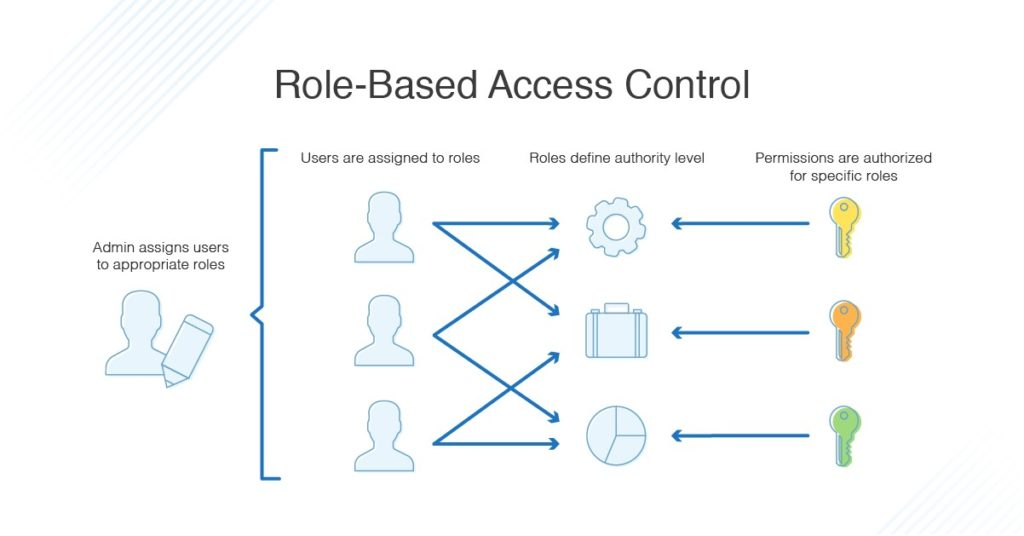
\includegraphics[width=.9\linewidth]{./img/rbac.jpg}
\caption{\label{fig:org8cfd3d4}RBAC}
\end{figure}

\label{org03a534b} - модель контроля доступа, в которой доступ к операции  производится на основании того, содержит ли роль субъекта соответствующую привилегию.

Роль - множество привилегий, доступных пользователям, которым присвоены соответсвующие роли.

Субъекту может быть присвоено несколько (0\ldots{}n) ролей. Роли может быть присвоено несколько привилегий (возможностей исполнить операцию) и/или объектов.
\end{block}



\begin{block}{ABAC (Attribute-Based Access Control)}
\label{org4cc13c0} - модель контроля доступа, в которой во внимание принимаются свойства (атрибуты) субъекта или объекта, а также свойства окружения (дата, время доступа).

\begin{center}
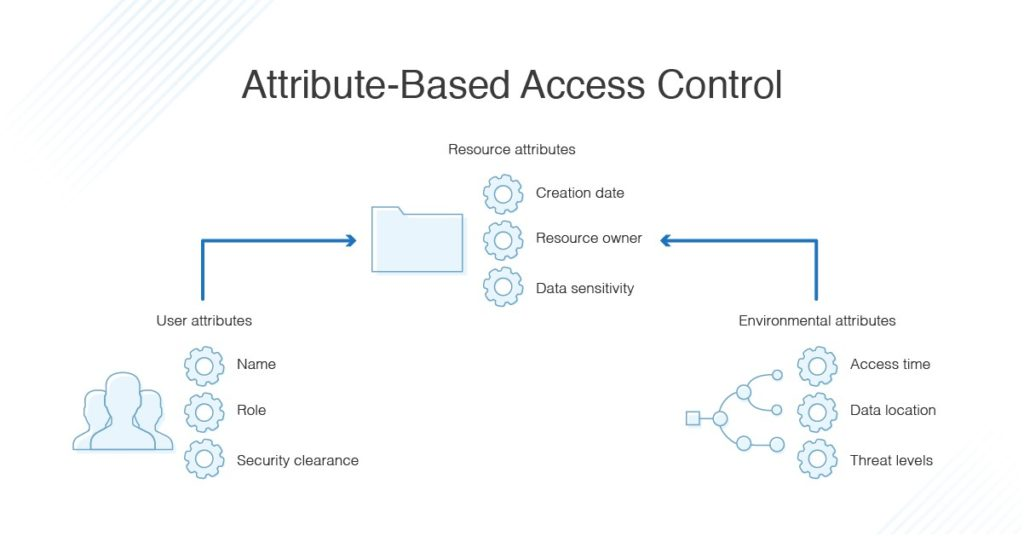
\includegraphics[width=.9\linewidth]{./img/abac.jpg}
\end{center}

Например:
\begin{itemize}
\item Пользователь(sub) может просмотреть документ(obj), если он(obj) создан коллегами из того же департамента
\item Пользователь(sub) может редактировать документ(obj), если он(subj) создал его(obj) и установлен режим черновика(obj).
\end{itemize}
\end{block}

\begin{block}{PERM}
Policy, Effect, Request, Matchers.
\end{block}
\end{frame}



\begin{frame}[label={sec:orga7be39e}]{Авторизация}
\begin{block}{OAuth 2.0}
Повсеместно используемое решение для авторизации - OAuth 2.0

Работает следующим образом:

\begin{center}
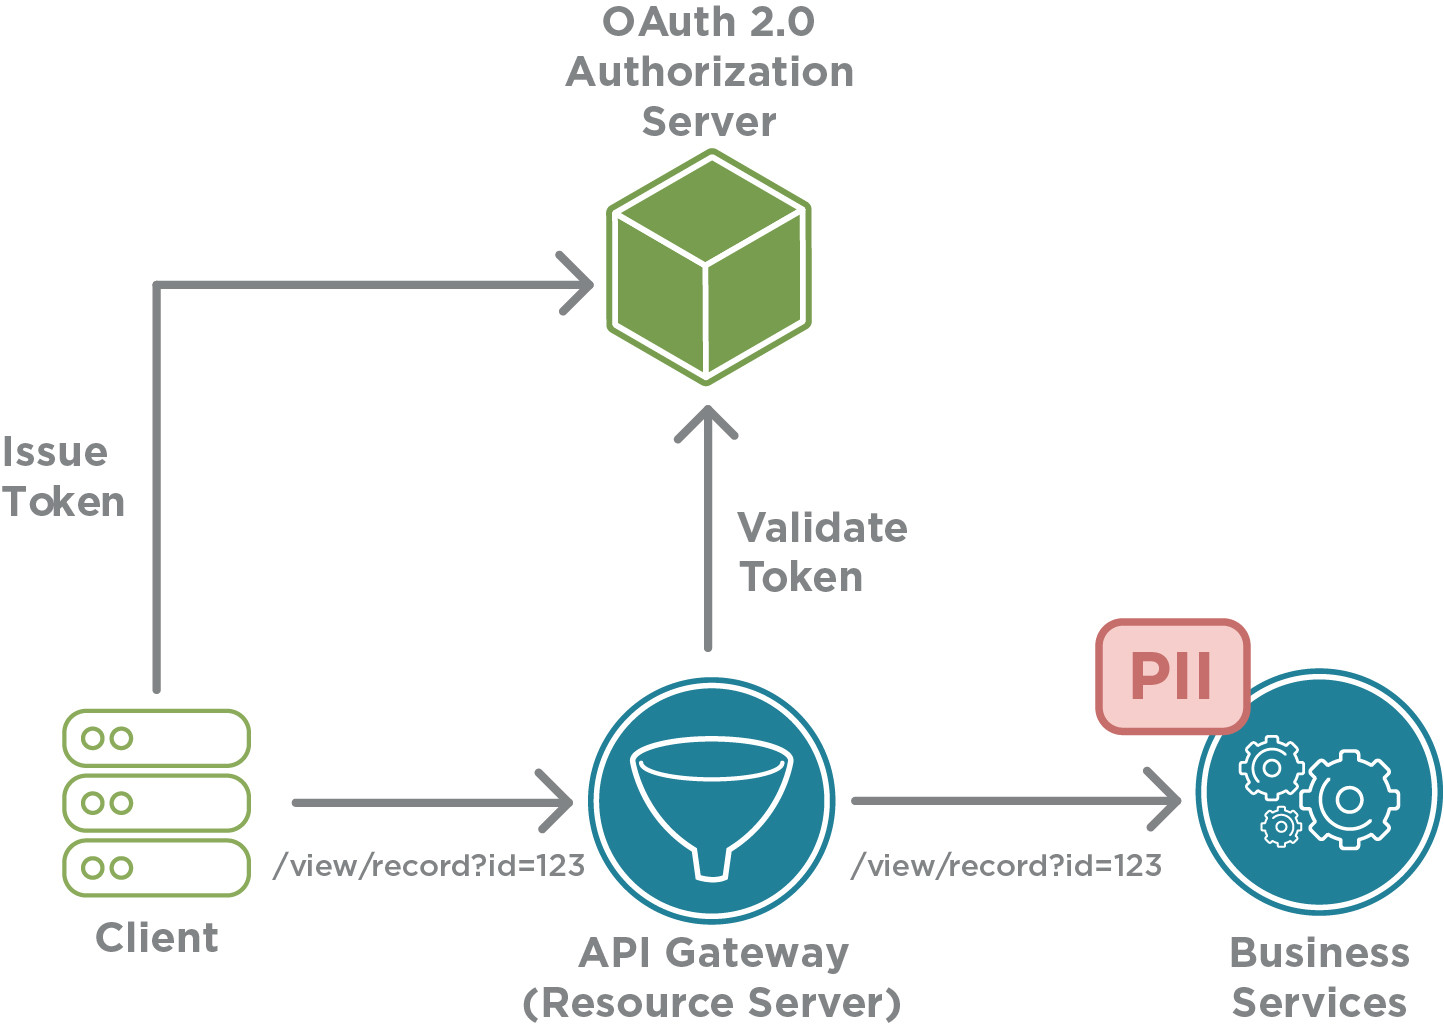
\includegraphics[width=.9\linewidth]{./img/oauth2.jpg}
\end{center}


\begin{enumerate}
\item Client посылает запрос к Authorization Server (AS)
\item Если Client не залогинен (кука нет или не валидный)
\begin{enumerate}
\item AS выдает форму логина и проверяет, что пользователь вошел правильно.
Источник пользователей - откуда угодно (DB, LDAP, etc)
\end{enumerate}
\item AS возвращает некоторый Token
\item API Gateway видит запрос с Token
\item API Gateway отправляет Token на AS
\item Если Token верный, AS одобряет.
\end{enumerate}


Доступ к отдельным объектам (Entities) в такой модели регулируется протоколом UMA:

\begin{center}
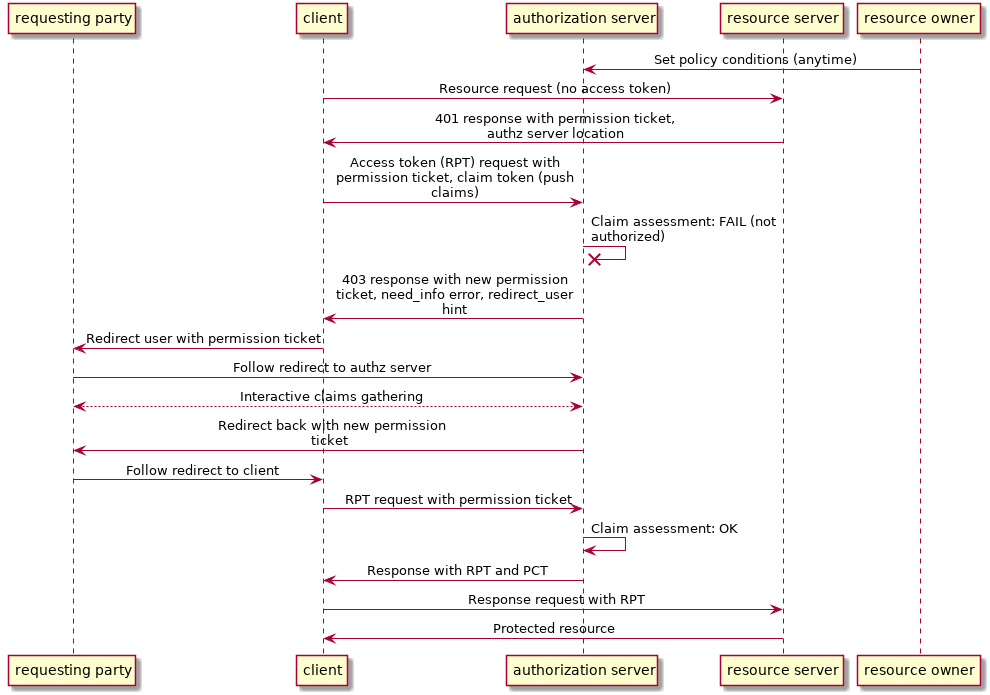
\includegraphics[width=.9\linewidth]{img/uma.png}
\end{center}

\begin{block}{Определения на схеме:}
\begin{itemize}
\item Requesting party - браузер
\item client - клиент, который хочет получить доступ к определенному ресурсу (часть веб-приложения или сам requesting party)
\item RPT - requesting party token - токен доступа OAuth
\item permission - авторизация доступа к определенному ресурсу с некоторому набором прав (scopes), привязанных к ресурсу
\item permission ticket - handle, представляющий запрошенные права доступа (permissions), необходимый в запросах к серверу авторизации
\item claim - запрос, представляющий требуемые атрибуты запрашиваемого ресурса/ов.
\item persisted claims token - токен, позволяющий много раз использовать набор claims для авторизации.
\end{itemize}
\end{block}
\end{block}
\end{frame}


\begin{frame}[label={sec:org90289dd},fragile]{Предлагаемое решение: Shiro}
 \begin{block}{Плюсы}
\begin{itemize}
\item \hyperlink{sec:org9c63c5e}{Модульная архитектура} - позволяет подключить OAuth2, если это будет нужно (например, если приложение авторизации будет лишь авторизирующим микросервисом)
\item Возможность регулировки доступа вплоть до отдельной записи в БД:
\end{itemize}
\begin{verbatim}
//Если выдать permission troopers:update:0, то обновлять штурмовика №0 будет можно
@PostMapping(path = "/{id}")
    public Stormtrooper updateTrooper(@PathVariable("id") String id, @RequestBody Stormtrooper updatedTrooper) throws NotFoundException {
        // Instance-based annotations are not supported, so we use direct check instead:
        SecurityUtils.getSubject().checkPermission(String.format("troopers:update:%s", id));
        return trooperDao.updateStormtrooper(id, updatedTrooper);
    }

\end{verbatim}
\end{block}

\begin{block}{Минусы}
\begin{itemize}
\item Медленная проверка permissions - O(n) в худшем случае:
\end{itemize}

\begin{block}{Обработка permissions по умолчанию (выдержка из исходного кода)}
\begin{verbatim}
//visibility changed from private to protected per SHIRO-332
 protected boolean isPermitted(Permission permission, AuthorizationInfo info) {
     Collection<Permission> perms = getPermissions(info);
     if (perms != null && !perms.isEmpty()) {
         for (Permission perm : perms) {
             if (perm.implies(permission)) {
                 return true;
             }
         }
     }
     return false;
 }
\end{verbatim}


Исправление: perm.implies использует wildcards. Возможно, стоит использовать более хитрую схему с хэш-таблицей (впрочем, данная реализация все равно единоразово подгружает все в память)

Источник данных JDBC реализован в классе JDBCRealm и его можно изменить

Кроме того, можно реализовать свой класс Permission, как показано \href{https://www.baeldung.com/apache-shiro-access-control}{здесь}.
\end{block}

\begin{block}{Нет решения для аггрегации всех ресурсов по permission}
Задал соответствующий вопрос \href{http://shiro-user.582556.n2.nabble.com/Using-Shiro-for-permission-based-resource-lookup-td7582096.html}{здесь.}
\end{block}
\end{block}
\begin{block}{Демо-проект}
\url{https://github.com/pashazz/shiro-example}

База данных штурмовиков из Звездных Войн. Сами штурмовики хранятся в памяти (hardcoded)

\begin{itemize}
\item Использует Spring Boot
\item Информация о пользователях в файле src/main/resources/shiro-users.properties
\item В данном примере вы сможете обновить штурмовика \#0 с помощью пользователя jcoder, но других - не сможете
\end{itemize}

\begin{block}{shiro-users.properties}
\begin{verbatim}
# Пользователи начинаются с user.
# Сначала идет пароль, потом роли через запятую


user.root = secret,admin
user.emperor = secret,emperor
user.officer = secret,officer
user.jcoder = secret,underling

# Роли начинаются с role.
# Роли поддерживают wildcards
# Можно разрешить действия только на объектах с определенным id
role.emperor = *
role.admin = troopers:*
role.officer = troopers:create, troopers:read, troopers:update
role.underling = troopers:read, troopers:update:0
\end{verbatim}
\end{block}
\end{block}
\end{frame}

\begin{frame}[label={sec:orga905e3a}]{Другие ссылки по теме}
\begin{itemize}
\item про реализацию RBAC на Rest \url{https://cloudify.co/blog/simple-secure-role-based-access-control-rest-api-rbac-server-devops-cloud-orchestration/}
\item Filter output: \url{https://www.baeldung.com/spring-security-role-filter-json}
\item ABAC with spring security: \url{https://dzone.com/articles/simple-attribute-based-access-control-with-spring}
\end{itemize}
\end{frame}
\end{document}